\documentclass{article}
\usepackage[UTF8]{ctex}
\usepackage{geometry}
\usepackage{natbib}
\geometry{left=3.18cm,right=3.18cm,top=2.54cm,bottom=2.54cm}
\usepackage{graphicx}
\pagestyle{plain}	
\usepackage{setspace}
\usepackage{caption2}
\usepackage{datetime} %日期
\renewcommand{\today}{\number\year 年 \number\month 月 \number\day 日}
\renewcommand{\captionlabelfont}{\small}
\renewcommand{\captionfont}{\small}
\begin{document}

\begin{figure}
    \centering
    
\includegraphics[width=8cm]{upc.png}

    \label{figupc}
\end{figure}

	\begin{center}
		\quad \\
		\quad \\
		\heiti \fontsize{45}{17} \quad \quad \quad 
		\vskip 1.5cm
		\heiti \zihao{2} 《计算科学导论》课程总结报告
	\end{center}
	\vskip 2.0cm
		
	\begin{quotation}
% 	\begin{center}
		\doublespacing
		
        \zihao{4}\par\setlength\parindent{7em}
		\quad 

		学生姓名:\underline{\qquad  张三 \qquad \qquad}

		学\hspace{0.61cm} 号:\underline{\qquad 190701xxxx\qquad}
		
		专业班级:\underline{\qquad 计科1901 \qquad  }
		
        学\hspace{0.61cm} 院:\underline{计算机科学与技术学院}
% 	\end{center}
		\vskip 2cm
		\centering
		\begin{table}[h]
            \centering 
            \zihao{4}
            \begin{tabular}{|c|c|c|c|c|c|c|}
            % 这里的rl 与表格对应可以看到,姓名是r,右对齐的;学号是l,左对齐的;若想居中,使用c关键字。
                \hline
                课程认识 & 问题思 考 & 格式规范  & IT工具  & Latex附加  & 总分 & 评阅教师 \\
                30\% & 30\% & 20\% & 20\% & 10\% &  &  \\
                \hline
                 & & & & & &\\
                & & & & & &\\
                \hline
            \end{tabular}
        \end{table}
		\vskip 2cm
		\today
	\end{quotation}

\thispagestyle{empty}
\newpage
\setcounter{page}{1}
% 在这之前是封面,在这之后是正文
\section{引言}
这里是一段引言。

\section{对计算科学导论这门课程的认识、体会}
总体说明你的整体认识,再举一、二个例子,从某个角度进一步展开讨论,以支持你的认识。\par

\subsection{这里是子标题样例}
图片插入的样例:\par
\begin{figure}[h!]
\centering
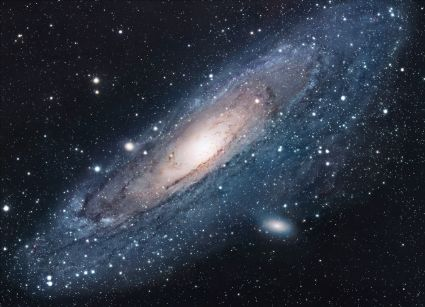
\includegraphics[scale=1.7]{universe}
\caption{The Universe}
\label{fig:universe}
\end{figure}

\subsection{第二个子标题}
表格插入样例:\par

\begin{table}[h]
    \centering
    \caption{这是科学系的花名册}
\begin{tabular}{rl}
% 这里的rl 与表格对应可以看到,姓名是r,右对齐的;学号是l,左对齐的;若想居中,使用c关键字。
    \hline
    姓名 & 学号 \\
    \hline
    张三 & 190704xxxx+++ \\ 
    李四 & 190704yyyy \\
    王二五 & 190704zzzz\\
    \hline
\end{tabular}
    \label{table1}
\end{table}
\subsection{第三个子标题}
这里是引用的样例:\par
{\bf 注意,仅仅是引用的样例}\par
我阅读了图书《机器学习实战》\citep{Harrington2013},引发了我对卷积神经网络的兴趣,于是阅读了期刊论文《卷积神经网络研究综述》\citep{zhoufeiyan},基于对卷积神经网络的深刻认识,我又学习了2018年计算机视觉领域的会议ECCV的会议论文《TextSnake》\citep{long2018textsnake},来探索深度学习落实在生活生产领域的实际意义。\par

\section{进一步的思考}
结合学习的计算科学知识,对分组演讲涉及的问题作进一步的思考。\par

这里是简单列表的样例:(如果需要标号自定义或者自动标记数字序号,请自行搜索语法)
\begin{itemize}
    \item 简单的列表结构 
    \item 如这里所示
    \item 此处仅为样例
    \item 按需修改和使用
\end{itemize}


\section{总结}
在这里,写自己对于整个课程和或本次报告的总结。\par


\section{附录}
\begin{itemize}
    \item 申请Github账户,给出个人网址和个人网站截图
    \item 注册观察者、学习强国、哔哩哔哩APP,给出对应的截图
    \item 注册CSDN、博客园账户,给出个人网址和个人网站截图
    \item 注册小木虫账户,给出个人网址和个人网站截图
\end{itemize}


\hspace*{\fill} \\

{\bf 注意,参考文献至少五篇,其中至少两篇为英文文献,参考文献必须在正文中有引用。}
\bibliographystyle{plain}
\bibliography{references}


\end{document}
